%%%%%%%%%%%%%%%%%%%%%%%%%%%%%%%%%%%%%%%%%%%%%%%%%%%%%%%%%%%%%%%%%%%%%
%
% CSCI 1430 Writeup Template
%
% This is a LaTeX document. LaTeX is a markup language for producing
% documents. Your task is to fill out this
% document, then to compile this into a PDF document.
% You will then upload this PDF to `Gradescope' - the grading system
% that we use.
%
%
% TO COMPILE:
% > pdflatex thisfile.tex
%
% For references to appear correctly instead of as '??', you must run
% pdflatex twice.
%
% If you do not have LaTeX and need a LaTeX distribution:
% - Departmental machines have one installed.
% - Personal laptops (all common OS): www.latex-project.org/get/
%
% If you need help with LaTeX, please come to office hours.
% Or, there is plenty of help online:
% https://en.wikibooks.org/wiki/LaTeX
%
% Good luck!
% James and the 1430 staff
%
%%%%%%%%%%%%%%%%%%%%%%%%%%%%%%%%%%%%%%%%%%%%%%%%%%%%%%%%%%%%%%%%%%%%%
%
% How to include two graphics on the same line:
%
% \includegraphics[\width=0.49\linewidth]{yourgraphic1.png}
% \includegraphics[\width=0.49\linewidth]{yourgraphic2.png}
%
% How to include equations:
%
% \begin{equation}
% y = mx+c
% \end{equation}
%
%%%%%%%%%%%%%%%%%%%%%%%%%%%%%%%%%%%%%%%%%%%%%%%%%%%%%%%%%%%%%%%%%%%%%%%%%%%%%%%%%%%%%%%%%%%%%%%%

\documentclass[11pt]{article}

\usepackage[english]{babel}
\usepackage[utf8]{inputenc}
\usepackage[colorlinks = true,
            linkcolor = blue,
            urlcolor  = blue]{hyperref}
\usepackage[a4paper,margin=1.5in]{geometry}
\usepackage{stackengine,graphicx}
\usepackage{fancyhdr}
\setlength{\headheight}{15pt}
\usepackage{microtype}
\usepackage{times}
\usepackage{booktabs}


\frenchspacing
\setlength{\parindent}{0cm} % Default is 15pt.
\setlength{\parskip}{0.3cm plus1mm minus1mm}

\pagestyle{fancy}
\fancyhf{}
\lhead{Image filtering project}
\rhead{CIE 552}
\rfoot{\thepage}

\date{}

\title{\vspace{-1cm}Hybrid image illusion using convolutional filtering}

\usepackage{listings}
\usepackage{color}

\definecolor{codegreen}{rgb}{0,0.6,0}
\definecolor{codegray}{rgb}{0.5,0.5,0.5}
\definecolor{codepurple}{rgb}{0.58,0,0.82}

\lstdefinestyle{mystyle}{
    commentstyle=\color{codegreen},
    keywordstyle=\color{magenta},
    numberstyle=\tiny\color{codegray},
    stringstyle=\color{codepurple},
    basicstyle=\footnotesize,
    breakatwhitespace=false,
    breaklines=true,
    captionpos=b,
    keepspaces=true,
    numbers=left,
    numbersep=5pt,
    showspaces=false,
    showstringspaces=false,
    showtabs=false,
    tabsize=2
}

\lstset{style=mystyle, language=python , frame=single}

\begin{document}

\maketitle	

\vspace{-3cm}
\thispagestyle{fancy}


\section*{Introduction}


Human eye's perception depends strongly on the distance between the object and the observer. If the distance was small, the eye start focusing more on the sharp details of the image (high frequency),however at the far away distances, the eye is only capable of detecting sooth variations (low frequency).In this project we are trying to use that phenomena to create an illusion by making hybrid image, which gets its low frequency content from an image and its high frequency content from another one.


\section*{Implementation of the convolutional filter}

This function is used to perform convolution operation over RGB and gray scale image . It has two types of padding (zeros and mirror).It takes only odd shaped kernel,and returns the output in the form of an image with the same size as the input image

\begin{lstlisting}
def my_imfilter(image, kernel,mode ='zeros'):
	# get the kernel dimesnsions in kh and kw
	kh,kw=kernel.shape
	# get the hight and width only as the third dimension may exist or not
	ih=image.shape[0]
	iw=image.shape[1]
	# get the number of dimsensions for both the kernel and the image
	kdim=kernel.ndim
	idim=image.ndim
	
	assert kdim == 2 , "kernel dimensions must be exaxctly two"
	assert idim == 2 or idim ==3 , "image dimensions must be exaxctly two or three"
	assert (kh%2) !=0 and (kw%2) !=0 , "all kernel dimensions must be odd"
	# this foarmula calculates how many rows do i need to put so that i can make proper padding
	hpad=(kh-1)//2
	wpad=(kw-1)//2
	
	filtered_image = np.zeros_like(image)
	
	if mode=='zeros':
		md='constant'
	elif mode=='reflect':
		md='reflect'
	else:
		raise   Exception('the mode {} is not defined \n "zeros" and "reflect are available"'.format(x))
	# change the padding function according to the input image
	if idim==2:
		paddedImg=np.pad(image,[(hpad,hpad),(wpad,wpad)],mode=md)
	else:
		paddedImg=np.pad(image,[(hpad,hpad),(wpad,wpad),(0,0)],mode='constant')
		dim_No=image.shape[2]
	# apply convolution over the number of channels
	for dim in range(0,dim_No):
		for i in range(0,ih):
			for j in range(0,iw):
				# multiply the kernel with the cropped part of the image and then sum the result
				
				cropped=paddedImg[i:i+kh,j:j+kw,dim]
				filtered_image[i,j,dim]=np.sum(np.multiply(kernel,cropped))
	
	return filtered_image

\end{lstlisting}

\section*{Filter tests and results}

{\Large \textbf{Identity filter}}

\begin{figure}[h]
    \centering
%    
\includegraphics[width=5cm]{placeholder.jpg}
%    
\includegraphics[width=5cm]{placeholder.jpg}
    \caption{\emph{Left:} My result was spectacular. \emph{Right:} Curious.}
    \label{fig:result1}
\end{figure}




\newpage
\section*{Generation of Hybrid Image}
In this part we are trying to add a low-pass filtered image and then add it to a high-pass filtered image of the same shape. This was implemented using 2 ways of filtering the first used the spatial convolution of the filter and the latter was done in frequency domain. The good thing of the frequency domain thing is that the convolution becomes a normal multiplication. 

The kernel used is a Gaussian kernel with size 15x15 and $\sigma = 10$.
This is how the low-pass filtered image was obtained and the high-filtered images was obtained by subtracting the low frequencies from the original image and this kept only high frequencies. 



Here is a code snippet of the function implemented 2 times one with spatial convolution and the second using FFT-based convolution


\begin{lstlisting}

def gen_hybrid_image(image1, image2, cutoff_frequency):
	
	assert image1.shape == image2.shape
	
	ksize = 15
	sigma = cutoff_frequency
	
	
	# Here I do outer product of 2 gaussian vectors to get 2D kernel
	x = np.arange(-ksize//2, ksize//2+1)
	gx = np.exp(-(x)**2/(2*sigma**2))
	g = np.outer(gx, gx)
	g /= np.sum(g)
	kernel = g
	
	
	
	# Your code here:
	# looping over the channels of the image to apply the gaussian kernel
	low_frequencies = np.zeros(image1.shape, dtype=np.float32)
	
	for i in range(image1.shape[2]):
	low_frequencies[:,:,i] = correlate2d(image1[:,:,i], kernel, 'same') # Replace with your implementation
	
	# (2) Remove the low frequencies from image2. The easiest way to do this is to
	#     subtract a blurred version of image2 from the original version of image2.
	#     This will give you an image centered at zero with negative values.
	
	low_frequencies2 = np.zeros(image2.shape, dtype=np.float32)
	
	for i in range(image1.shape[2]):
	low_frequencies2[:,:,i] = correlate2d(image2[:,:,i], kernel,'same')
	
	
	
	
	
	high_frequencies = image2 - low_frequencies2 # Replace with your implementation
	
	
	# print(np.sum(high_frequencies<0))
	
	# (3) Combine the high frequencies and low frequencies
	
	hybrid_image = low_frequencies/2 + high_frequencies/2 # Replace with your implementation
	
	high_frequencies = np.clip(high_frequencies,-1.0,1.0)
	hybrid_image = np.clip(hybrid_image,0,1)

	# np.clip(low_frequencies,0,1)
	# np.clip(high_frequencies,0,1)
	# np.clip(hybrid_image,0,1)
	return low_frequencies, high_frequencies, hybrid_image


\end{lstlisting}

\newpage
	
\begin{lstlisting}
def gen_hybrid_image_fft(image1, image2, cutoff_frequency):
	assert image1.shape == image2.shape
	
	ksize = 15
	sigma = cutoff_frequency
	
	x = np.arange(-ksize//2, ksize//2+1)
	gx = np.exp(-(x)**2/(2*sigma**2))
	g = np.outer(gx, gx)
	g /= np.sum(g)
	kernel = g
	
	
	# Applyingthe fft convolution on each channel
	low_freqs = np.zeros(image1.shape)
	for i in range(image1.shape[2]):
	low_freqs[:,:,i] = fft_convolve(image1[:,:,i], kernel)
	
	
	
	low_freqs2 = np.zeros(image2.shape)
	for i in range(image1.shape[2]):
	low_freqs2[:,:,i] = fft_convolve(image2[:,:,i], kernel)
	
	
	# getting only high freqs of image2
	high_freqs = image2 - low_freqs2
	
	
	# combining the low freqs and high freqs
	hybrid_image = low_freqs/2 + high_freqs/2 # Replace with your implementation
	
	high_freqs = np.clip(high_freqs,-1.0,0.5)
	hybrid_image = np.clip(hybrid_image,0,1)
	
	return low_freqs, high_freqs, hybrid_image


\end{lstlisting}
\newpage

\section{Results}
The code worked perfectly in both spatial and FFT-based convolution.


Here are the 2 images I used:

low Frequencies
\begin{figure}[h]
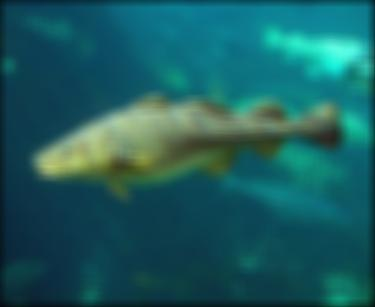
\includegraphics{../results/low_frequencies}
\label{fig:low frequencies}
\end{figure}

\newpage
High Frequncies
\begin{figure}[h]
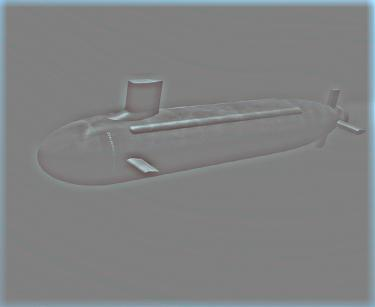
\includegraphics{../results/high_frequencies}
\end{figure}

\newpage
Both added together
\begin{figure}[h]
	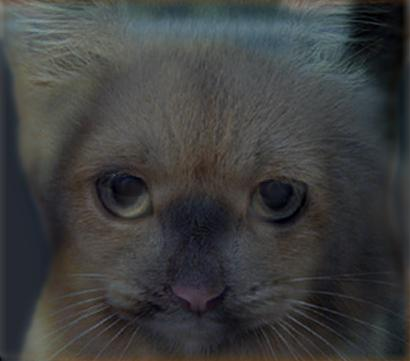
\includegraphics{../results/hybrid_image}
\end{figure}


\newpage
And here it is on different scales
\begin{figure}[h]
	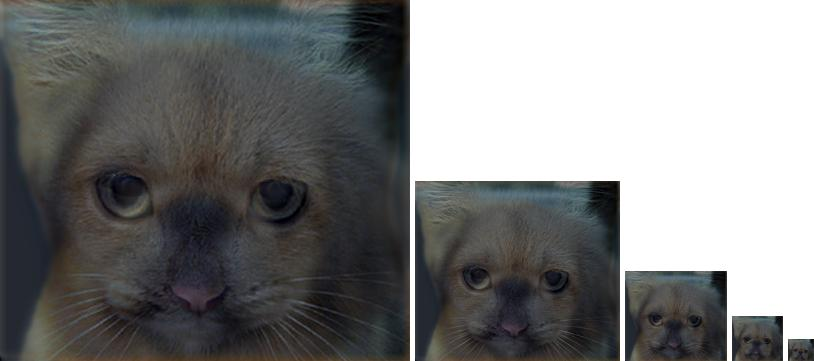
\includegraphics[scale=0.6]{../results/hybrid_image_scales}
\end{figure}





\end{document}
